% Template for MEng/BEng/MSc final reports
% EEE Department - Imperial College London
% Compile with LuaLaTeX + Biber

\documentclass[10pt]{ic_eee_thesis}

\usepackage[style=ieee,backend=biber,hyperref=auto]{biblatex}
\addbibresource{references.bib}

%%%%%%%%%%%%%%%% SETUP %%%%%%%%%%%%%%%%
% Degree
%\degree{MEng}
%\degree{BEng}
\degree{MSc}

\title{Predicting the Expansion of \textit{Parthenium hysterophorus} Under Climate Change Scenarios: Environmental and spatial drivers of \textit{Parthenium} invasion across agroecosystems in South Asia}
\subtitle{}
\author{Anaga Ambady}
\cid{00000000}
\supervisor{Anaga Ambady}
\submityear{2026}

% Course
%\course{Analogue and Digital Integrated Circuit Design}
%\course{Applied Machine Learning}
%\course{Communications and Signal Processing}
\course{Control and Optimisation}
%\course{Future Power Networks}

% Front matter options
\setboolean{list_of_figures}{true}
\setboolean{list_of_tables}{true}
\setboolean{acknowledgement}{true}
\setboolean{acronyms}{false}
\setboolean{edge_labels}{true}
\setboolean{double_spacing}{true}

% MSc ignores Part B settings, but template may still define them harmlessly
\setboolean{final_thesis}{true}
\secondmarker{}

%%%%%%%%%%%%%%%% ADDITIONAL PACKAGES %%%%%%%%%%%%%%%%
\usepackage{amsmath}
\usepackage{amsfonts}
\usepackage{booktabs}
\usepackage{graphicx}
\usepackage{float}
\usepackage{caption}
\usepackage{subcaption}
\usepackage{longtable}
\usepackage{array}
\usepackage{multirow}
\usepackage{pdflscape}
\usepackage{csquotes}
\usepackage{setspace}

%%%%%%%%%%%%%%%% ADDITIONAL COMMANDS %%%%%%%%%%%%%%%%
\DeclareMathOperator{\diag}{diag}
\DeclareMathOperator{\vect}{vec}

\begin{document}

\preamble

% Front matter files to edit inside chapters/
% chapters/Abstract.tex
% chapters/OrigSta_Copyright.tex
% chapters/Acknowledgement.tex

% Additional front matter required by programme guidance
\input{chapters/Declaration.tex}

% Main dissertation chapters
\chapter{Introduction}

\section{Parthenium as an invasive alien plant species}

Invasive alien plant species (IAPS) pose severe threats to South Asian biodiversity, agriculture, and human health, with \textit{Parthenium hysterophorus} among the most aggressive invaders [X]. Native to the Americas, this annual herb, commonly known as ``Congress grass'' or ``Gajar Booti'', has rapidly colonised diverse habitats across Asia, Africa, and Australia [X]. Its success stems from high phenotypic plasticity, allelopathic suppression, and broad tolerance, together with a persistent soil seed bank capable of surviving wide thermal ranges [X]. Despite decades of spread since its mid-twentieth-century introduction to South Asia [X], key gaps remain regarding how microclimate, human dispersal, and land-use changes interact to drive its expansion. This study investigates the spatiotemporal spread of \textit{P. hysterophorus} in India and Pakistan, mapping environmental and anthropogenic drivers to address management gaps and inform biosecurity policy [X].

Parthenium exemplifies a fast-maturing annual plant characterised by a deep taproot and an erect stem. Most individuals remain below 1.5 m in height, although some may reach up to 2.5 m [X]. The small, white flowers (approximately 4 mm in diameter) display five distinct lobes, and each plant is capable of producing up to 20{,}000 viable seeds from its 2 mm wedge-shaped achenes [X]. The soil seed bank may contain over 340 million seeds per hectare. Rapid proliferation during germination, combined with fast growth and allelopathic properties, enables \textit{Parthenium} to establish strongly, suppress neighbouring vegetation, and maintain a persistent seed bank [X].

\section{Introducing the spread of parthenium weed in South Asia}

\textit{Parthenium hysterophorus} was likely introduced into India in the 1950s through contaminated PL 480 wheat shipments from the United States, initially appearing as stray plants in Pune [X]. Although records from 1814 suggest earlier localised occurrences, large-scale expansion began in the mid-twentieth century [X]. By 1972, the weed had spread from Kashmir to Kerala, and by 1979 it had reached Assam. It now occurs in every Indian state, with Karnataka alone accounting for approximately 5 million hectares of infestation [X]. In Pakistan, \textit{Parthenium} was first confirmed in the Gujrat district of Punjab in 1980, likely entering through cross-border trade at the Wagah border [X]. It subsequently spread across Punjab, Khyber Pakhtunkhwa (KP), Islamabad Capital Territory (ICT), and Azad Jammu and Kashmir, with severe infestations concentrated in central and northern Punjab, ICT, and KP, and the invasion continuing southward [X]. \textit{Parthenium} now occurs throughout South Asia and is among the region's most problematic weeds.

This dissertation examines the environmental, climatic, and anthropogenic factors underlying the transition of \textit{P. hysterophorus} from localised introductions to widespread subcontinental invasion. Understanding these drivers is essential for explaining its ecological impacts and the persistent challenges of containment across South Asia.

\textit{Parthenium} spreads through both natural and human-mediated pathways [X]. Farmers identify water and vehicles as major dispersal agents, while wind, animals, and contaminated agricultural products facilitate movement of its lightweight seeds [X]. Human-mediated transport enables the species to overcome barriers such as rivers, mountains, and climatic zones. This study therefore investigates the dispersal dynamics and transport networks, including road hierarchies, that facilitate its regional spread.

Despite extensive management efforts, including mechanical removal, chemical herbicides, competitive replacement, and biological control, \textit{Parthenium} remains highly invasive. Prolific seed production, a persistent soil seed bank, rapid growth, broad ecological tolerance, and the ability to exploit disturbed habitats promote rapid establishment. Through allelopathy and competition for resources, it suppresses native vegetation, reducing biodiversity and promoting dense monocultures. These traits are particularly advantageous across South Asia's agricultural land, grazing areas, roadsides, and other disturbed habitats.

The region's warm climate, seasonal rainfall, extensive agriculture, and habitat disturbance further facilitate establishment and persistence. In India and Pakistan, cultivated landscapes, irrigation, livestock movement, transport corridors, and degraded habitats form interconnected pathways for dispersal. Together, these environmental and anthropogenic factors have enabled the rapid expansion of \textit{P. hysterophorus} across South Asia, highlighting the need to understand the mechanisms sustaining its invasion.

\section{Harmful effects of \textit{Parthenium hysterophorus}}

\textit{Parthenium hysterophorus} rapidly colonises disturbed habitats, including wastelands, roadsides, waterways, and agricultural fields, across a wide range of environmental conditions. Prolific seed production, rapid growth, and broad climatic tolerance enable it to form dense stands that displace native species and disrupt ecosystem processes. Disturbance, rainfall, and temperature influence its distribution and impacts in South Asia, while land-use change and soil disturbance further enhance persistence and agricultural impacts through allelopathy and competition for resources.

Human activity, particularly agriculture and transportation, also drives its spread and exposure. Rural communities and agricultural workers are disproportionately affected, as infestations frequently occur around cultivated land and transport networks. Exposure to the plant's allergenic compounds can cause dermatitis and respiratory conditions, including bronchitis. Increasing land use and connectivity therefore amplify risks to both agricultural production and public health [X].

The impacts of \textit{P. hysterophorus} extend across interconnected ecological, agricultural, and socioeconomic systems. These effects are particularly pronounced in South Asia, where high population density, agricultural dependence, and favourable environmental conditions facilitate rapid spread and exposure. Consequently, \textit{P. hysterophorus} represents not only an ecological invasion but also a significant agricultural, economic, and public health concern, reinforcing the need for integrated regional management.

\section{Biocontrol management and climate expansion}

Long-term management of \textit{Parthenium hysterophorus} remains challenging due to its adaptability and ongoing expansion. Rising atmospheric CO$_2$ may further increase herbicide resistance, necessitating a reassessment of traditional control strategies. Climate change is projected to facilitate additional spread of \textit{Parthenium} and other invasive species, amplifying the urgency for proactive management.

Species distribution models reinforce these risks: CLIMEX analyses indicate much of South Asia is already suitable for \textit{Parthenium} establishment. Climate change scenarios predict continued northward expansion, with irrigation and warming enabling colonisation of previously unsuitable regions. Identifying high-risk areas will be essential for targeted monitoring and early intervention. Control methods, including burning, herbicides, and biological agents such as beetles, moths, weevils, and fungi, have yielded variable results. The biocontrol beetle \textit{Zygogramma bicolorata}, for example, is highly sensitive to temperatures above 35$^{\circ}$C, complicating sustainable management as climate warms [X].

\section{Study aims}

Despite extensive research, major gaps remain, particularly concerning cross-border dynamics and climate-driven changes in distribution. India and Pakistan are considered together here because of their shared invasion history, contiguous borders, and differing climates and agricultural systems that distinctly influence \textit{Parthenium}'s distribution. However, comparative region-wide analyses are scarce, limiting understanding of how climate change may affect both \textit{Parthenium} and its biocontrol beetle across these countries.

This study models current and projected distributions of \textit{Parthenium} and its biocontrol beetle across India and Pakistan, integrating occurrence records with environmental variables. It hypothesises that climate change will alter both distributions, with direct management implications. By identifying emerging invasion risks and changes in habitat suitability, this research highlights where management, especially biological control, must adapt, guiding proactive strategies for vulnerable regions.
\chapter{Methods}

\section{Study design and modelling framework}

This study examined environmental and spatial drivers of \textit{Parthenium hysterophorus} presence and projected its distribution under climate change. The analysis comprised four stages: (1) field surveys across Pakistan; (2) processing ERA5 climate data; (3) developing a fine-scale binomial Generalised Additive Model (GAM) for Pakistan; and (4) broader-scale presence-only modelling with MaxEnt to estimate climatic suitability and its overlap with the thermal suitability of the biocontrol agent \textit{Zygogramma bicolorata}. Candidate GAM and GLM structures were evaluated using the Pakistan survey data. A GAM was implemented as the primary fine-scale model, while MaxEnt provided a complementary presence-only framework for broader-scale projections.

\section{Field data collection in Pakistan}

Primary data were collected via systematic roadside surveys in Pakistan during four rounds (December 2018, March 2019, June 2019, October 2019) by CABI researchers. Surveys spanned different phenological stages and expanded from northern to southern Pakistan. The first two rounds focused on Khyber Pakhtunkhwa and Punjab; the latter two included Sindh. A stratified random sampling design was used at district, grid-cell, and site levels. Ten districts per province were selected, and 10 \texttimes{} 10 km grid cells were assessed based on ecological zone, agricultural context, and road accessibility. At each site, observations were recorded within a 20 \texttimes{} 20 m plot. Geographic coordinates were taken at the roadside and 20 m perpendicular to the road. Recorded variables included road type; habitat type and cover; \textit{P. hysterophorus} presence, phenological stage, and abundance; crop type; phenological stage; and irrigation method; together with relevant site observations. Road and habitat categories followed OpenStreetMap and Pakistan land-cover classifications. All data were recorded electronically using standardised ODK Collect forms.

\section{Climate data extraction and processing}

Climate covariates for the Pakistan GAM were derived from hourly ERA5-Land data using a Python workflow. Observation coordinates and dates were matched to the nearest ERA5 grid cell, with a 60-day look-back to verify coverage. Hourly temperature data were aggregated to daily means. Seven- and 30-day rolling means and growing degree days (GDD) were then calculated to represent recent germination and longer-term establishment conditions. GDD was estimated using a parabolic thermal-response function with \textit{P. hysterophorus}-specific thermal thresholds:

$$
T_{\mathrm{base}} = 7.2^{\circ}\mathrm{C}, \qquad T_{\mathrm{opt}} = 25^{\circ}\mathrm{C}, \qquad T_{\mathrm{max}} = 42.8^{\circ}\mathrm{C}
$$

Climate values were extracted for each observation date and location, assigning observations to the corresponding ERA5 grid cell. For the broader presence-only analysis, a separate R-based workflow generated 1991--2020 climate normals from monthly ERA5 data. Monthly values were averaged by calendar month to retain seasonal pattern while reducing interannual variability. Three predictors were derived: mean annual temperature (BIO1), total annual precipitation (BIO12), and temperature seasonality (BIO4). The same processing was applied to Pakistan projection layers to maintain consistency between model calibration and projection.

\section{Environmental and spatial drivers of \textit{Parthenium} presence in Pakistan}

\subsection{GAM structure}

A binomial GAM was fitted to the Pakistan presence--absence data using 30-day GDD and precipitation metrics, together with altitude, road type, habitat cover, habitat group, and a bivariate spatial smooth of longitude and latitude.

\subsection{Model selection}

Candidate models were compared using AIC, explained deviance, and spatial-block cross-validation to evaluate predictor structures and spatial resolutions. Specifically, candidate structures tested whether:

\begin{itemize}
    \item a habitat-specific GDD smooth improved model performance compared to a single pooled GDD smooth;
    \item road type contributed meaningful explanatory power regarding transport-corridor dispersal;
    \item a habitat-specific factor-smooth structure outperformed a shared-shape factor-smooth; and
    \item spatial smooth basis dimensions ($k = 100$ vs. $k = 200$) captured fine-scale spatial structure without overfitting.
\end{itemize}

\subsection{Final GAM specification}

The final model used a binomial family with a logit link and Restricted Maximum Likelihood (REML) smoothing-parameter selection. The model was specified as:

$$
\begin{aligned}
\text{presence} \sim {} & \text{hab\_group} + \text{road\_type} + \\
& s(\text{precip\_sum\_30d}, k=25) + s(\text{gdd\_30d}, k=25) + \\
& s(\text{gdd\_30d}, \text{by}=\text{hab\_group}, k=15) + s(\text{altitude}, k=15) + \\
& s(\text{hab\_perc}, k=10) + s(\text{longitude}, \text{latitude}, \text{bs}=\text{"gp"}, k=200)
\end{aligned}
$$

\section{Presence-only species distribution modelling for \textit{Parthenium hysterophorus}}

\subsection{Occurrence data and calibration area}

Indian occurrence records were obtained from GBIF (\texttt{parthenium\_india\_gbif.csv}). Duplicate and spatially redundant records were removed, followed by spatial thinning to reduce sampling clustering. Multiple thinning replicates were generated, selecting the replicate retaining the largest number of records. Records were restricted to the terrestrial area of India using GADM boundaries. The accessible calibration area ($M$) was defined by buffering each occurrence by 100 km, dissolving the buffers, and clipping the result to India to define a biologically informed calibration region.

\subsection{Climate predictors}

ERA5-Land monthly climatological data for 1991--2020 were used to derive mean annual temperature (MAT), total annual precipitation (TAP), and temperature seasonality:

$$
\text{MAT} = \text{mean}(t2m_{1:12}) - 273.15
$$

$$
\text{TAP} = \text{mean}(tp_{1:12}) \times 365.25 \times 1000
$$

$$
\text{Seasonality} = \text{sd}(t2m_{1:12})
$$

Predictors were clipped to the calibration area for model fitting and projection.

\subsection{Sampling bias and background selection}

Natural Earth road vectors were clipped to the calibration area, rasterised to the climate grid, and Gaussian-smoothed to construct a continuous bias surface representing sampling accessibility. Values were normalised to 0.0001--1, where higher values represented higher expected sampling effort. Using this surface, 10{,}000 background points were sampled without replacement from cells with valid weights, using a fixed random seed (42) for reproducibility.

\subsection{MaxEnt fitting and thresholding}

Cleaned occurrences, weighted background points, and climate predictors were combined for model fitting, excluding records with missing environmental data. Model complexity was optimised using ENMeval with four-block spatial cross-validation. Feature classes (L, LQ, and LQH) were evaluated alongside regularisation multipliers ranging from 0.5 to 4.0 (0.5 increments). The model with the lowest $\Delta\text{AICc}$ was selected and refitted on all calibration data. Current suitability was predicted using cloglog output, and a binary suitability map was generated using the 10th percentile training-presence threshold.

\subsection{Future projections}

The selected MaxEnt model was projected onto climate stacks representing 2030 and 2050 conditions using the identical predictor structure and calibration order to assess shifts in climatic suitability.

\section{Overlap with the biocontrol agent \textit{Zygogramma bicolorata}}

Potential overlap between \textit{P. hysterophorus} and \textit{Z. bicolorata} was assessed under current, 2030, and 2050 climate conditions. Plant suitability was extracted from MaxEnt projections. Beetle thermal suitability was estimated from mean annual temperature using a temperature-response function defined by:

$$
T_{\min} = 10^{\circ}\mathrm{C}, \qquad T_{\mathrm{opt}} = 27^{\circ}\mathrm{C}, \qquad T_{\max} = 38^{\circ}\mathrm{C}
$$

Suitability layers were aligned to a common grid and masked for terrestrial data. Continuous predictions were converted to binary suitability maps using predefined thresholds and classified into four categories: (1) neither suitable, (2) \textit{P. hysterophorus} only, (3) beetle only, and (4) both suitable. Area and class proportions were computed across periods.

Extreme heat effects were evaluated using a 2050 summer maximum-temperature raster, classifying areas into within tolerance, heat stress, or likely unsuitable categories.

\section{Transferability comparison between India-trained MaxEnt and Pakistan-trained GAM}

Transferability was evaluated by comparing the India-trained MaxEnt projection with the Pakistan-trained GAM across Pakistan. MaxEnt was projected using MAT, TAP, and temperature seasonality; GAM was projected using GDD, precipitation, altitude, and habitat cover.

Predictor layers were aligned to a common grid with categorical variables held at reference training levels. GAM predictions were restricted to environmental conditions represented in training data. Predictions were converted to percentile ranks (0 to 1) to establish a common relative scale, calculated as:

$$
\text{Rank difference} = \text{GAM rank} - \text{MaxEnt rank}
$$

Positive values indicated higher relative suitability predicted by GAM, whereas negative values indicated higher relative suitability by MaxEnt. High-suitability agreement was evaluated across the upper 25\% of predictions. Model concordance was quantified using Spearman's rank correlation, Pearson's correlation, Jaccard and S{\o}rensen indices, Cohen's kappa, and shared vs. model-specific hotspot proportions.
\chapter{Results}

\section{Environmental and spatial drivers of \textit{Parthenium hysterophorus} presence in Pakistan}

\subsection{Model selection}

Model selection showed that incorporating spatial structure substantially improved model performance (Table~\ref{tab:model-comparison}). The non-spatial model (M1\_noloc) explained just 38.17\% of the deviance and had the poorest fit, with an AIC 1678.86 units higher than the best-performing model. In contrast, models with a two-dimensional spatial smooth explained 55.37\% to 60.33\% of the deviance, highlighting the importance of spatial dependence.

Among REML-fitted models, increasing the spatial smooth basis from $k = 100$ (M4\_k100) to $k = 200$ (M5\_k200) produced the best model, reducing AIC by 207.83 units and raising explained deviance from 56.82\% to 60.33\%. Excluding altitude (M3\_xalt) substantially reduced model performance (AIC increased by 314.69 units; deviance explained fell to 55.37\%), demonstrating altitude's unique explanatory value beyond climatic and spatial predictors. Maximum-likelihood comparisons further supported retaining road type in the final model. Excluding road type (M7\_noroad) or its smooth interaction (M6\_noroad\_sm) significantly reduced model fit compared to the full model (M8\_full\_ml), with AIC increases of 19.04 units or more ($p < 0.001$). Thus, M5\_k200 was selected for further analyses, as it minimised AIC, maximised explanatory power, and included all ecologically relevant predictors.

Although basis-dimension diagnostics yielded $k$-index values below one for all spatial models (0.72--0.80; $p < 0.001$), increasing $k$ to 200 substantially improved model performance, justifying its use in the final model. A substantial residual spatial component remained after accounting for environmental, habitat, and road variables. The spatial Gaussian-process smooth was highly significant (edf = 109.80, $\chi^2$ = 977.85, $p < 0.001$), indicating spatial structure in occurrence beyond measured environmental predictors. Therefore, the spatial term was retained to account for geographically structured variation in occurrence rather than as an environmental driver.

\begin{table}[H]
    \centering
    \caption{Model comparison and goodness-of-fit evaluation across generalised additive model (GAM) candidate formulations. Models are fitted via Restricted Maximum Likelihood (REML) and evaluated based on Total Effective Degrees of Freedom (EDF), percentage deviance explained, Akaike Information Criterion (AIC), change in AIC relative to the best-performing model ($\Delta\text{AIC}$), likelihood-ratio test (LRT) $p$-values, and spatial basis-dimension adequacy ($k$-index and $p$-value from \texttt{k.check}). The primary full model (M5\_k200) is retained in red.}
    \label{tab:model-comparison}
    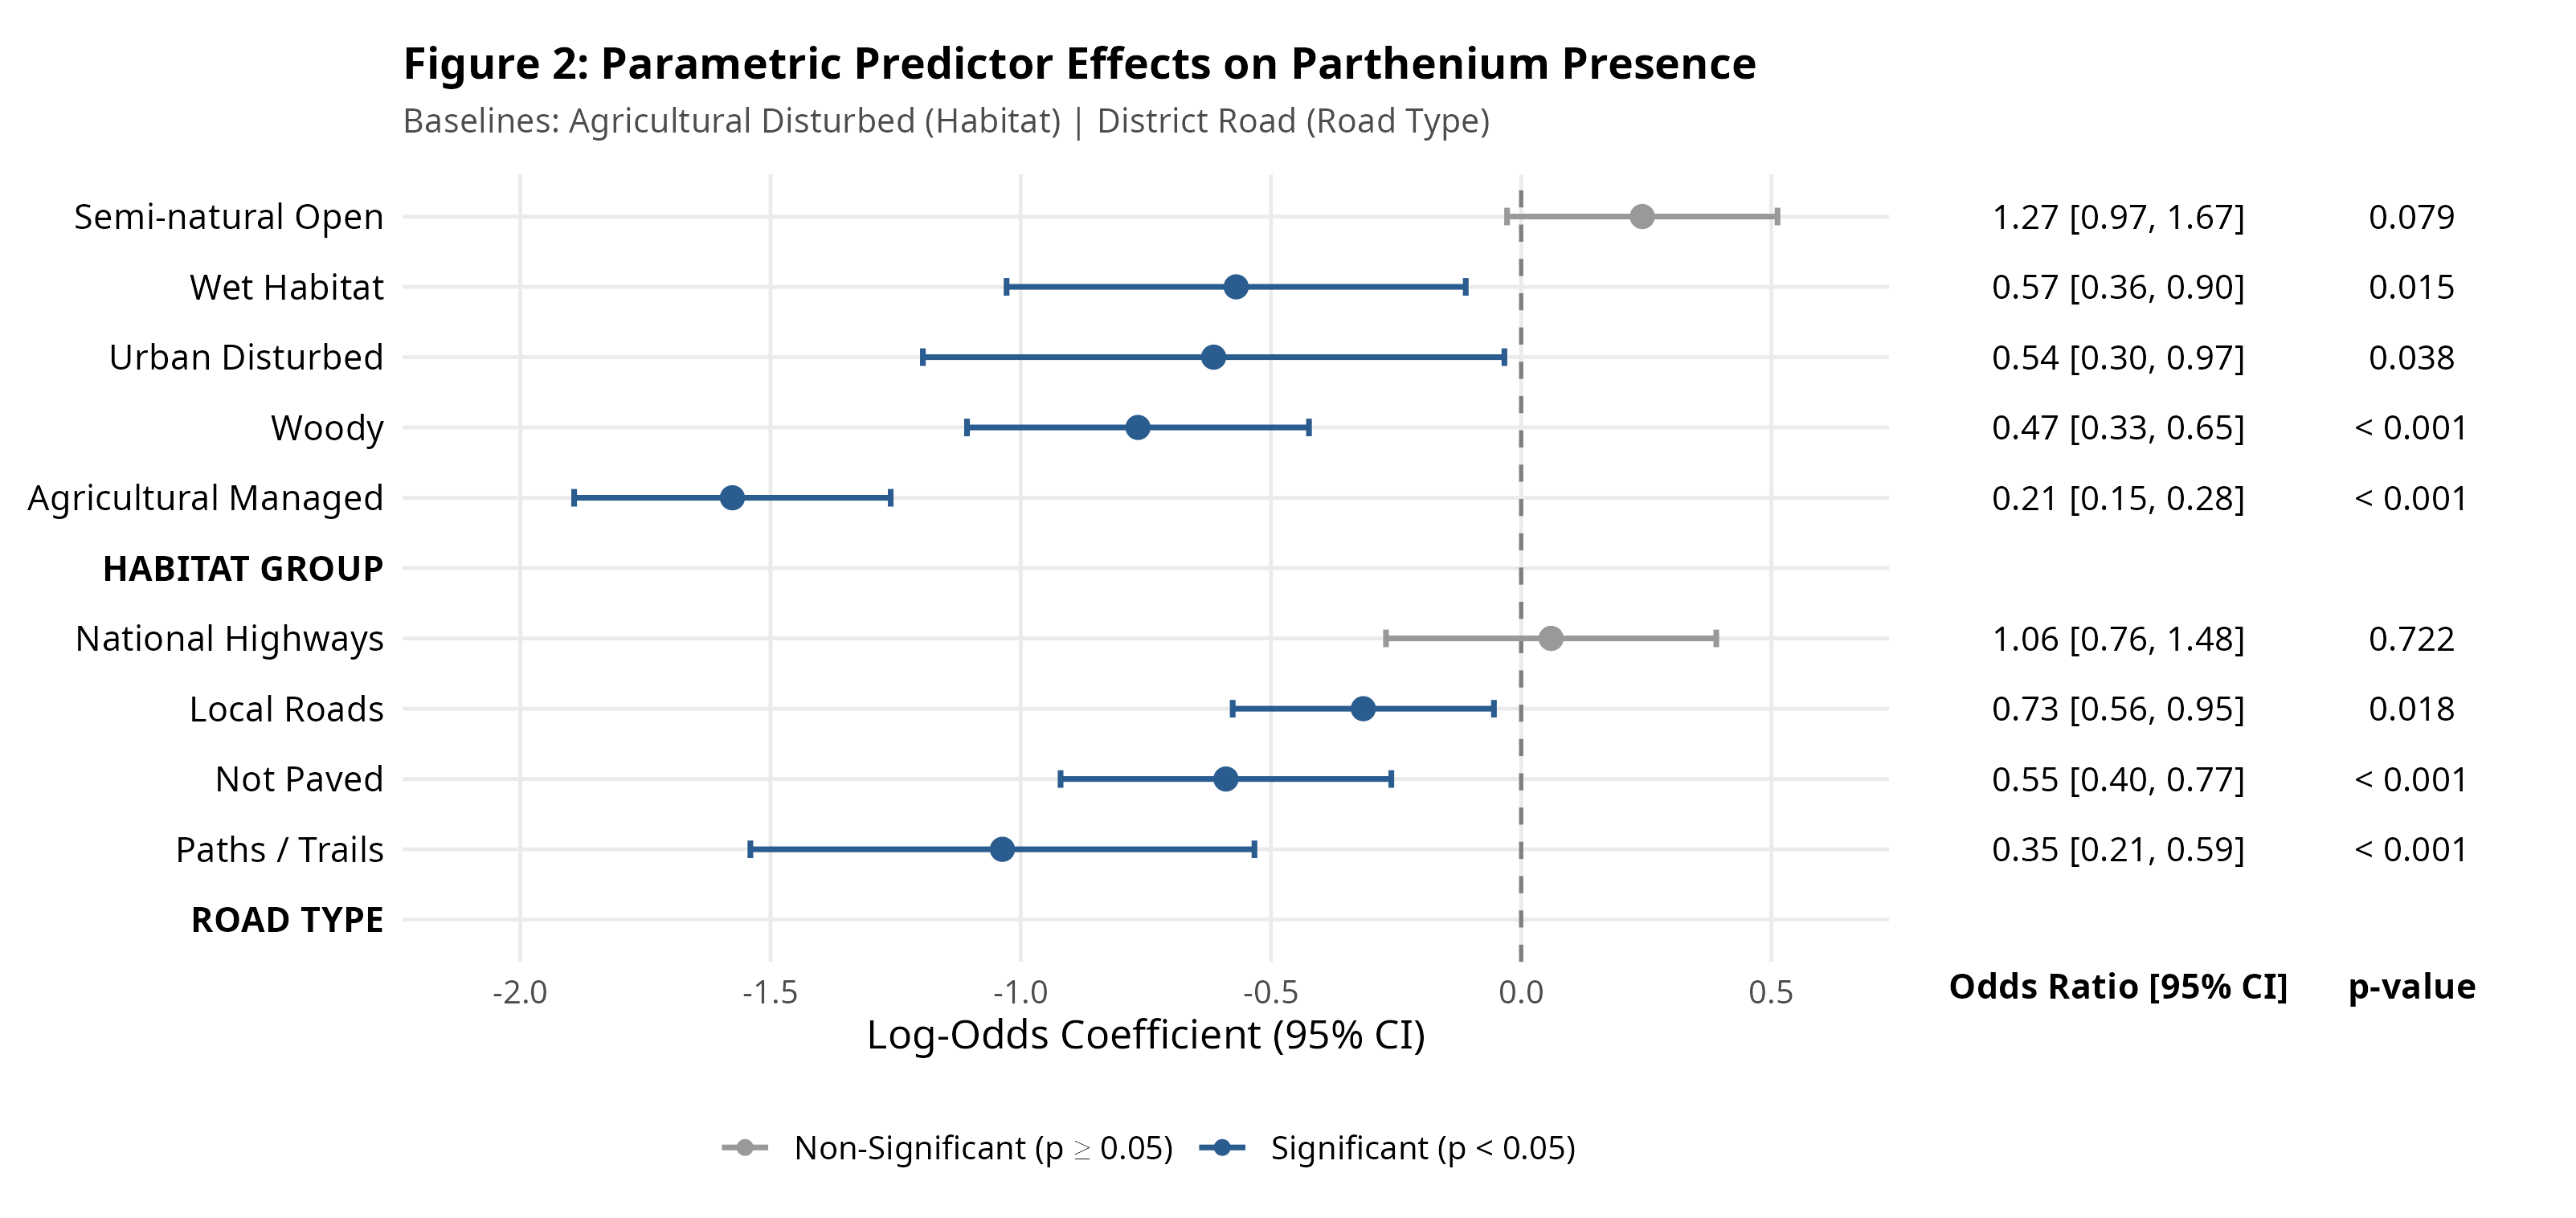
\includegraphics[width=\textwidth]{figures/fig2_parametric_forest_table.png}
\end{table}

\subsection{Final model performance}

The final REML-fitted GAM explained 60.33\% of the deviance in \textit{Parthenium hysterophorus} presence (adjusted $R^2 = 0.629$, REML = 2000.6, $n = 6{,}852$). The model included a bivariate spatial smooth (longitude, latitude), global smooths for cumulative temperature and growing degree days (GDD), habitat-specific smooths for GDD, altitude, habitat cover, habitat group, and road type.

The final model can be expressed as:

\begin{verbatim}
gam_gdd_k_200 <- gam(
  presence ~
    hab_group +
    road_type +
    s(precip_sum_30d, k = 25) +
    s(gdd_30d, k = 25) +
    s(gdd_30d, by = hab_group, k = 15) +
    s(altitude, k = 15) +
    s(hab_perc, k = 10) +
    s(longitude, latitude, bs = "gp", k = 200),
  family = binomial(link = "logit"),
  method = "REML",
  data = survey_data)
\end{verbatim}

Further analyses assessed the significance and functional form of smooth and parametric terms to identify key environmental and spatial drivers of \textit{P. hysterophorus} occurrence in Pakistan.

\section{Parametric effects of habitat and transport infrastructure}

Parametric fixed effects from the final GAM (M5\_k200) showed significant variation in \textit{P. hysterophorus} occurrence odds across habitat groups and road types (Figure~\ref{fig:parametric-effects}). Coefficients are reported as log-odds and odds ratios, relative to the Agricultural Disturbed habitat and District Road reference categories.

\subsection*{Habitat group}

Habitat group strongly influenced occurrence odds. All categories except Semi-natural Open differed significantly from the Agricultural Disturbed baseline ($p < 0.05$):

\begin{itemize}
    \item Semi-natural Open habitat had a positive but non-significant difference from disturbed agriculture ($\beta = 0.237$, SE = 0.138, $p = 0.084$), indicating similar or slightly higher occurrence probability in unmanaged open areas.
    \item Urban Disturbed ($\beta = -0.599$, OR = 0.55, $p = 0.043$), Wet Habitat ($\beta = -0.580$, OR = 0.56, $p = 0.013$), and Woody Vegetation ($\beta = -0.772$, OR = 0.46, $p < 0.001$) all showed significantly reduced odds of occurrence.
    \item Agricultural Managed land had the strongest negative effect, reducing occurrence odds by 79\% compared to disturbed agriculture ($\beta = -1.569$, OR = 0.21, $p < 0.001$).
\end{itemize}

\subsection*{Road type}

Occurrence odds declined along a gradient of decreasing road size, traffic volume, and accessibility (Figure~\ref{fig:parametric-effects}):

\begin{itemize}
    \item National Highways did not differ significantly from District Roads ($\beta = 0.039$, OR = 1.04, $p = 0.814$), indicating high occurrence probability along both major transport corridors.
    \item Lower-tier routes showed reduced occurrence odds: Local Roads ($\beta = -0.340$, OR = 0.71, $p = 0.010$) and Unpaved Roads ($\beta = -0.612$, OR = 0.54, $p < 0.001$).
    \item Paths and Trails had the largest reduction, lowering odds by 66\% compared to District Roads ($\beta = -1.077$, OR = 0.34, $p < 0.001$).
\end{itemize}

These results reveal a clear disturbance gradient: occurrence odds are highest in habitats and road types with the most disturbance and vehicular traffic (District Roads, National Highways, Agricultural Disturbed, Semi-natural Open). Odds decrease with greater disturbance suppression (Agricultural Managed, Woody habitat) or lower propagule delivery (Local, Unpaved Roads, Paths/Trails). This pattern aligns with the established ecology of \textit{P. hysterophorus} as a ruderal and disturbance-dependent species and supports the role of road networks and land management as primary drivers of \textit{P. hysterophorus} occurrence.

\begin{figure}[H]
    \centering
    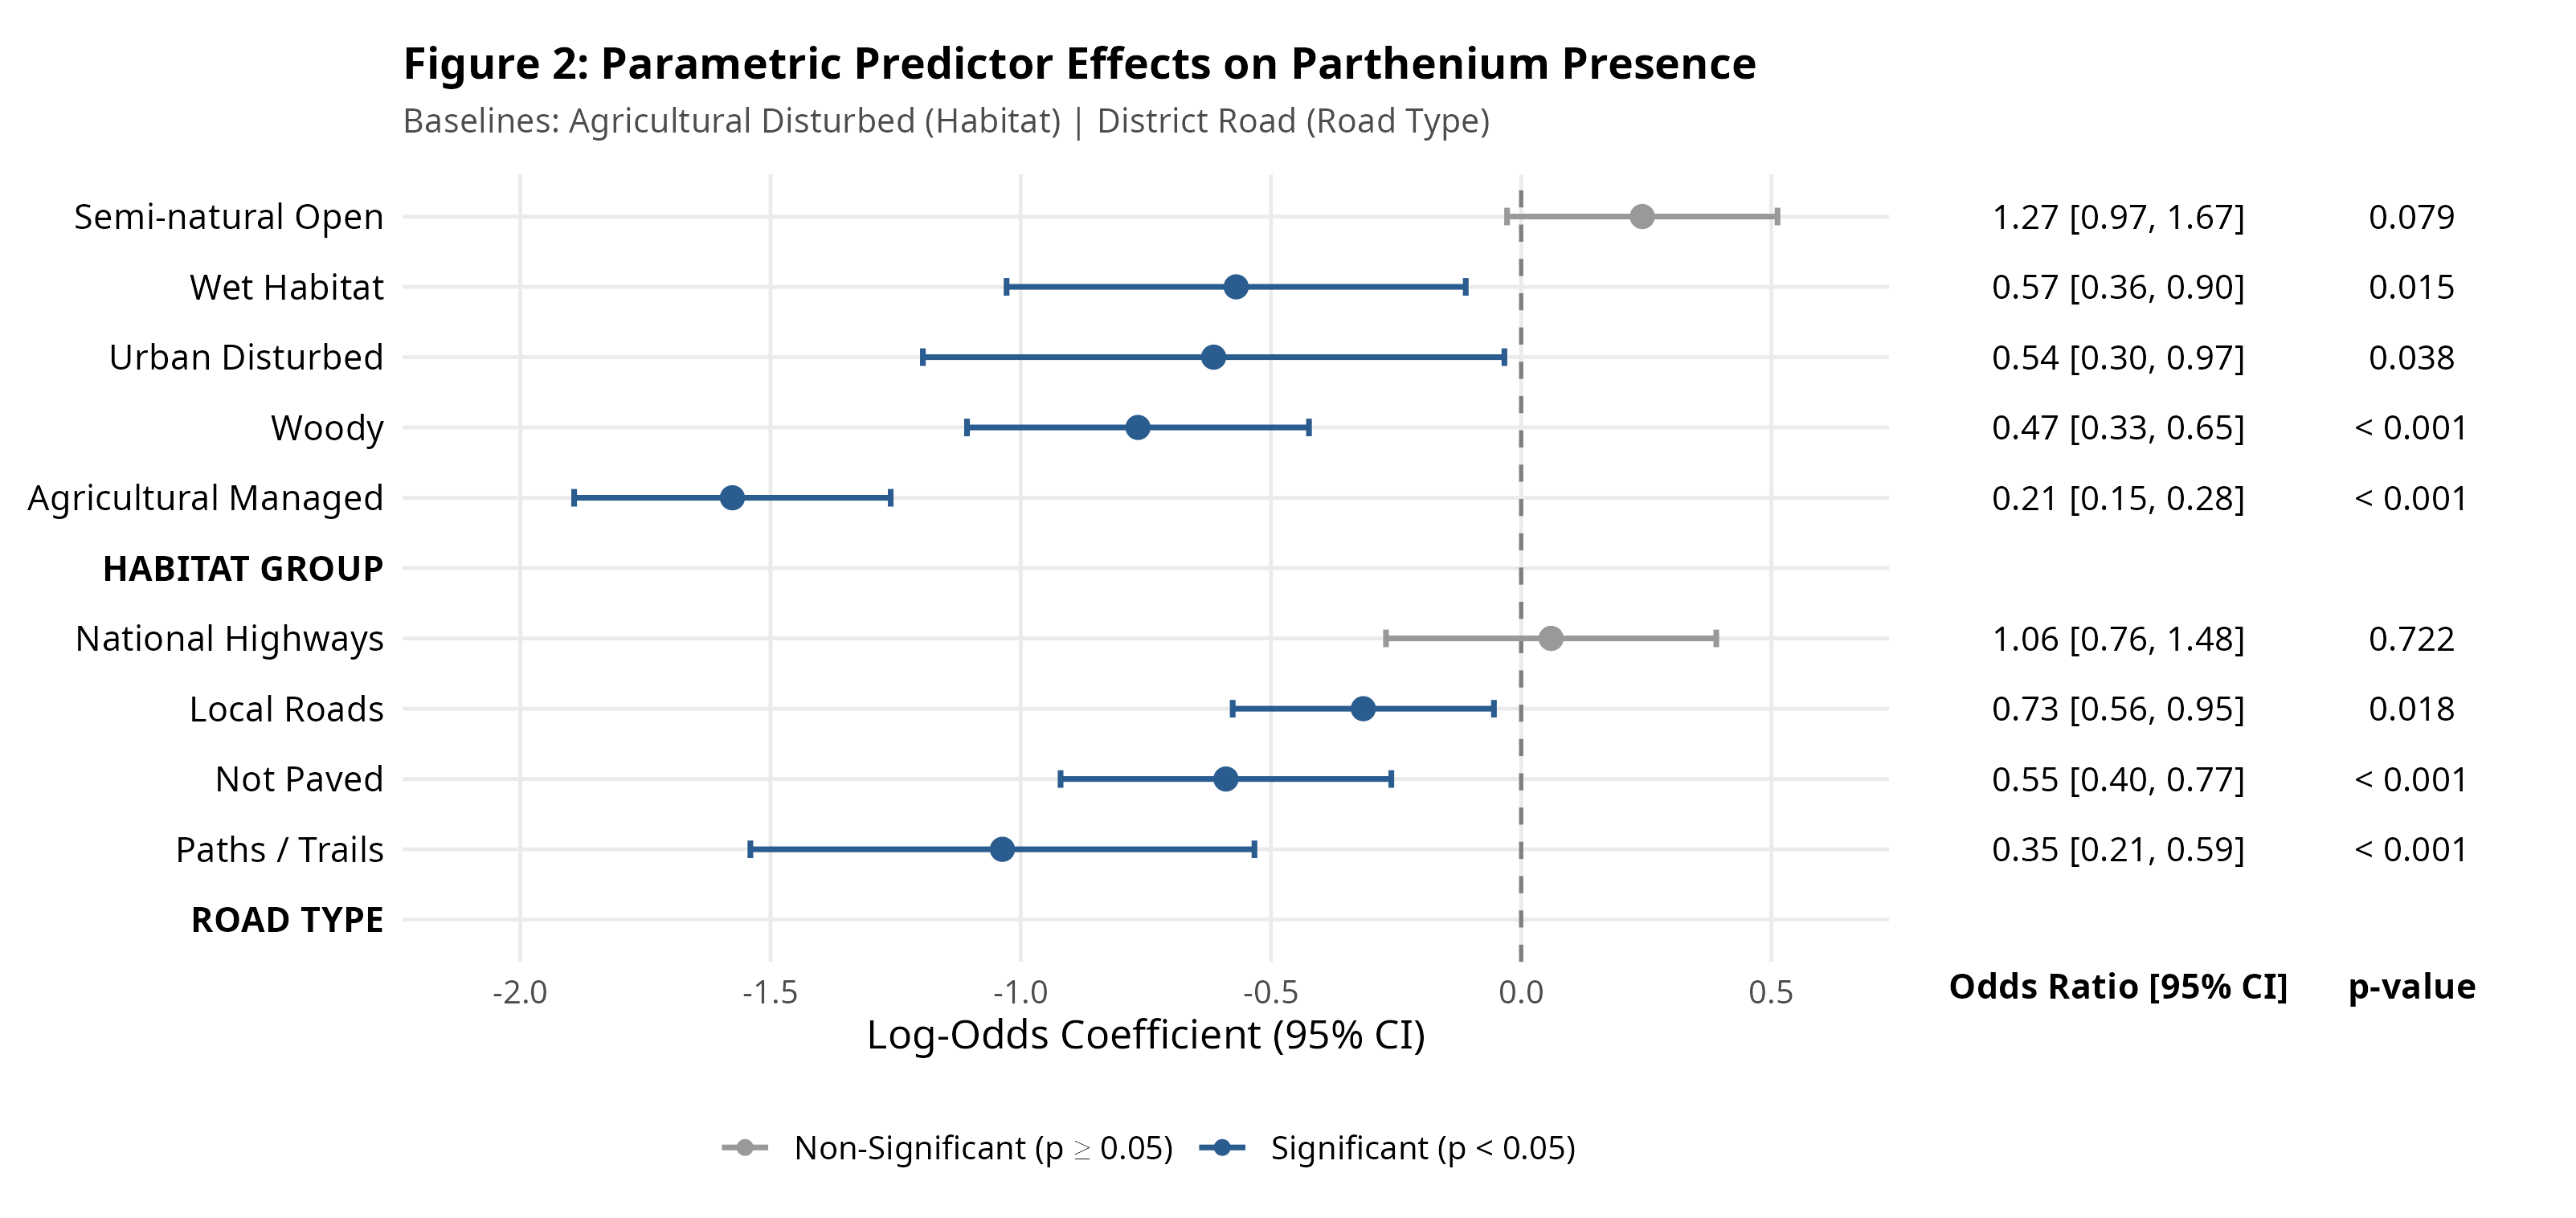
\includegraphics[width=\textwidth]{figures/fig2_parametric_forest_table.png}
    \caption{Parametric fixed effects on \textit{Parthenium hysterophorus} occurrence. Left panel: forest plot of log-odds coefficients (95\% confidence intervals) relative to baseline reference categories (Agricultural Disturbed for habitat; District Road for road classification). Points and error bars are colored by statistical significance (alpha = 0.05). Right panel: corresponding exponentiated odds ratios (OR = $e^{\beta}$) with 95\% confidence intervals and two-tailed $p$-values.}
    \label{fig:parametric-effects}
\end{figure}

\section{Non-linear climate responses across habitat types}

\subsection*{Regional thermal response: growing degree days (GDD)}

Growing degree days over the preceding 30 days (30dGDD) were a strong, non-linear predictor of \textit{Parthenium hysterophorus} occurrence. The global smooth was highly significant (edf = 11.51, $\chi^2$ = 81.26, $p < 0.001$), with diagnostics ($k' = 24$, $k$-index = 0.99) supporting genuine non-linearity rather than a modelling artefact.

Predicted occurrence was highest in Semi-natural Open and Agricultural Disturbed habitats and lowest in Agricultural Managed land, particularly across 200--750 30dGDD. In the less-managed habitats, occurrence probability peaked around 300 and 650--700 30dGDD (0.25--0.30), whereas Agricultural Managed habitats showed near-zero probability across the gradient (Figure~\ref{fig:gdd-response}).

Raw observations similarly indicated elevated occurrence at 50--150, 450--500, and particularly 600--750 30dGDD, followed by a decline above 750. However, sparse sampling at the gradient extremes and wide confidence intervals limit interpretation of these apparent peaks as biological thresholds.

Occurrence also varied seasonally, with presence rates highest in August and additional increases in November in some habitats, while February--March and October were lower. This pattern suggests the GDD response reflects seasonal phenology and habitat conditions rather than multiple physiological optima. Overall, 30dGDD was an important predictor, but occurrence is likely also shaped by precipitation, soil moisture, disturbance, vegetation structure, and land management.

\begin{figure}[H]
    \centering
    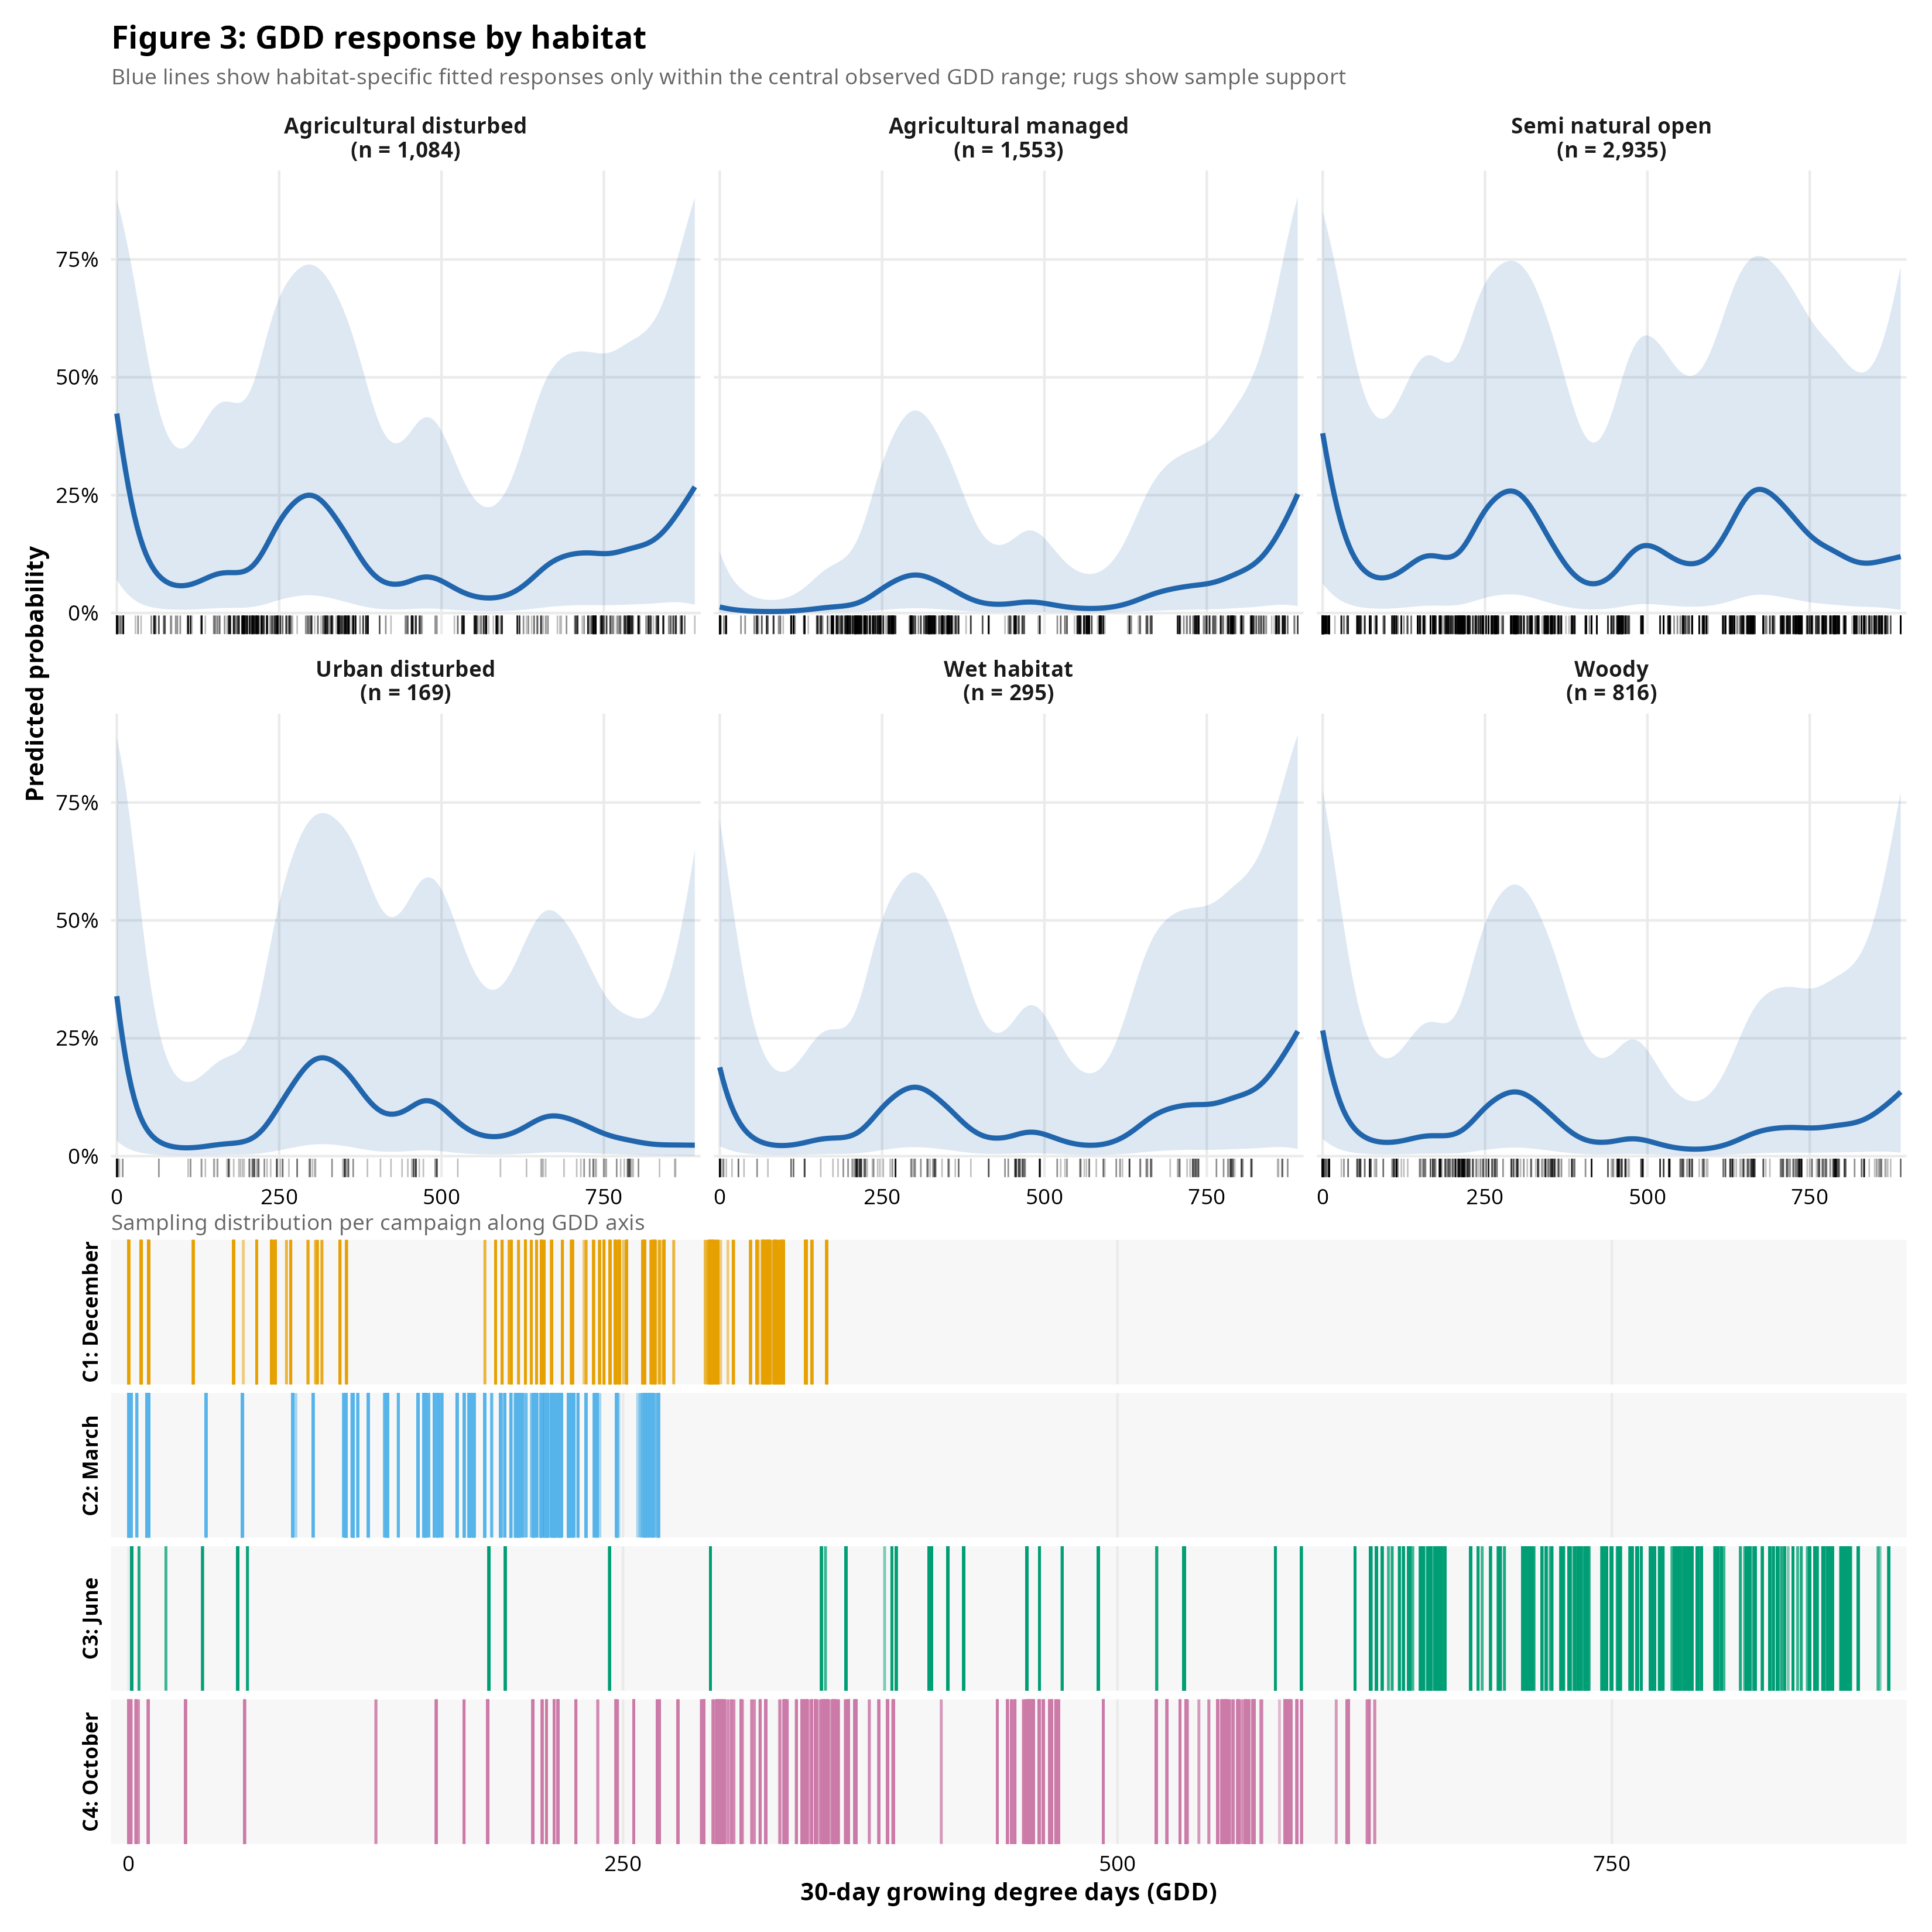
\includegraphics[width=\textwidth]{figures/fig3_with_campaign_rug.png}
    \caption{Non-linear response of \textit{Parthenium hysterophorus} occurrence probability to 30-day Growing Degree Days ($\text{GDD}_{30\text{d}}$) across habitat groups. Curves depict partial predictions from model \texttt{M5\_k200} holding spatial and secondary predictors constant. Shaded ribbons represent 95\% confidence intervals. Note that sharp probability increases and wide confidence ribbons at boundary extremes ($\text{GDD}_{30\text{d}} < 50$ and $> 800$) reflect sparse sampling density and spline boundary uncertainty.}
    \label{fig:gdd-response}
\end{figure}

\subsection*{Precipitation and other environmental predictors}

The relationship between 30-day cumulative precipitation and occurrence was nonlinear and highly significant (edf = 4.59, $\chi^2$ = 28.56, $p < 0.001$). Occurrence probability was highest at low to moderate precipitation, peaking at 50--120 mm and plateauing near 100 mm ($\approx 0.23$). As precipitation increased, probability declined, with greater uncertainty at the upper end of the range (Figure~\ref{fig:precip-response}).

Beyond 120 mm, occurrence probability declined sharply, approaching zero above 200 mm. This pattern matches the categorical habitat effect, with wet habitats showing lower occurrence than agricultural disturbed areas. Overall, moisture availability emerged as a key environmental correlate of \textit{P. hysterophorus} occurrence.

At very low precipitation ($< 25$ mm), the response curve rose slightly and confidence intervals widened, likely due to sparse sampling and hydrological effects such as irrigation or drainage. Altitude also showed a strong association with occurrence (edf = 5.25, $\chi^2$ = 56.94, $p < 0.001$), while habitat cover had a weaker but significant nonlinear effect (edf = 2.00, $\chi^2$ = 8.99, $p = 0.017$).

\begin{figure}[H]
    \centering
    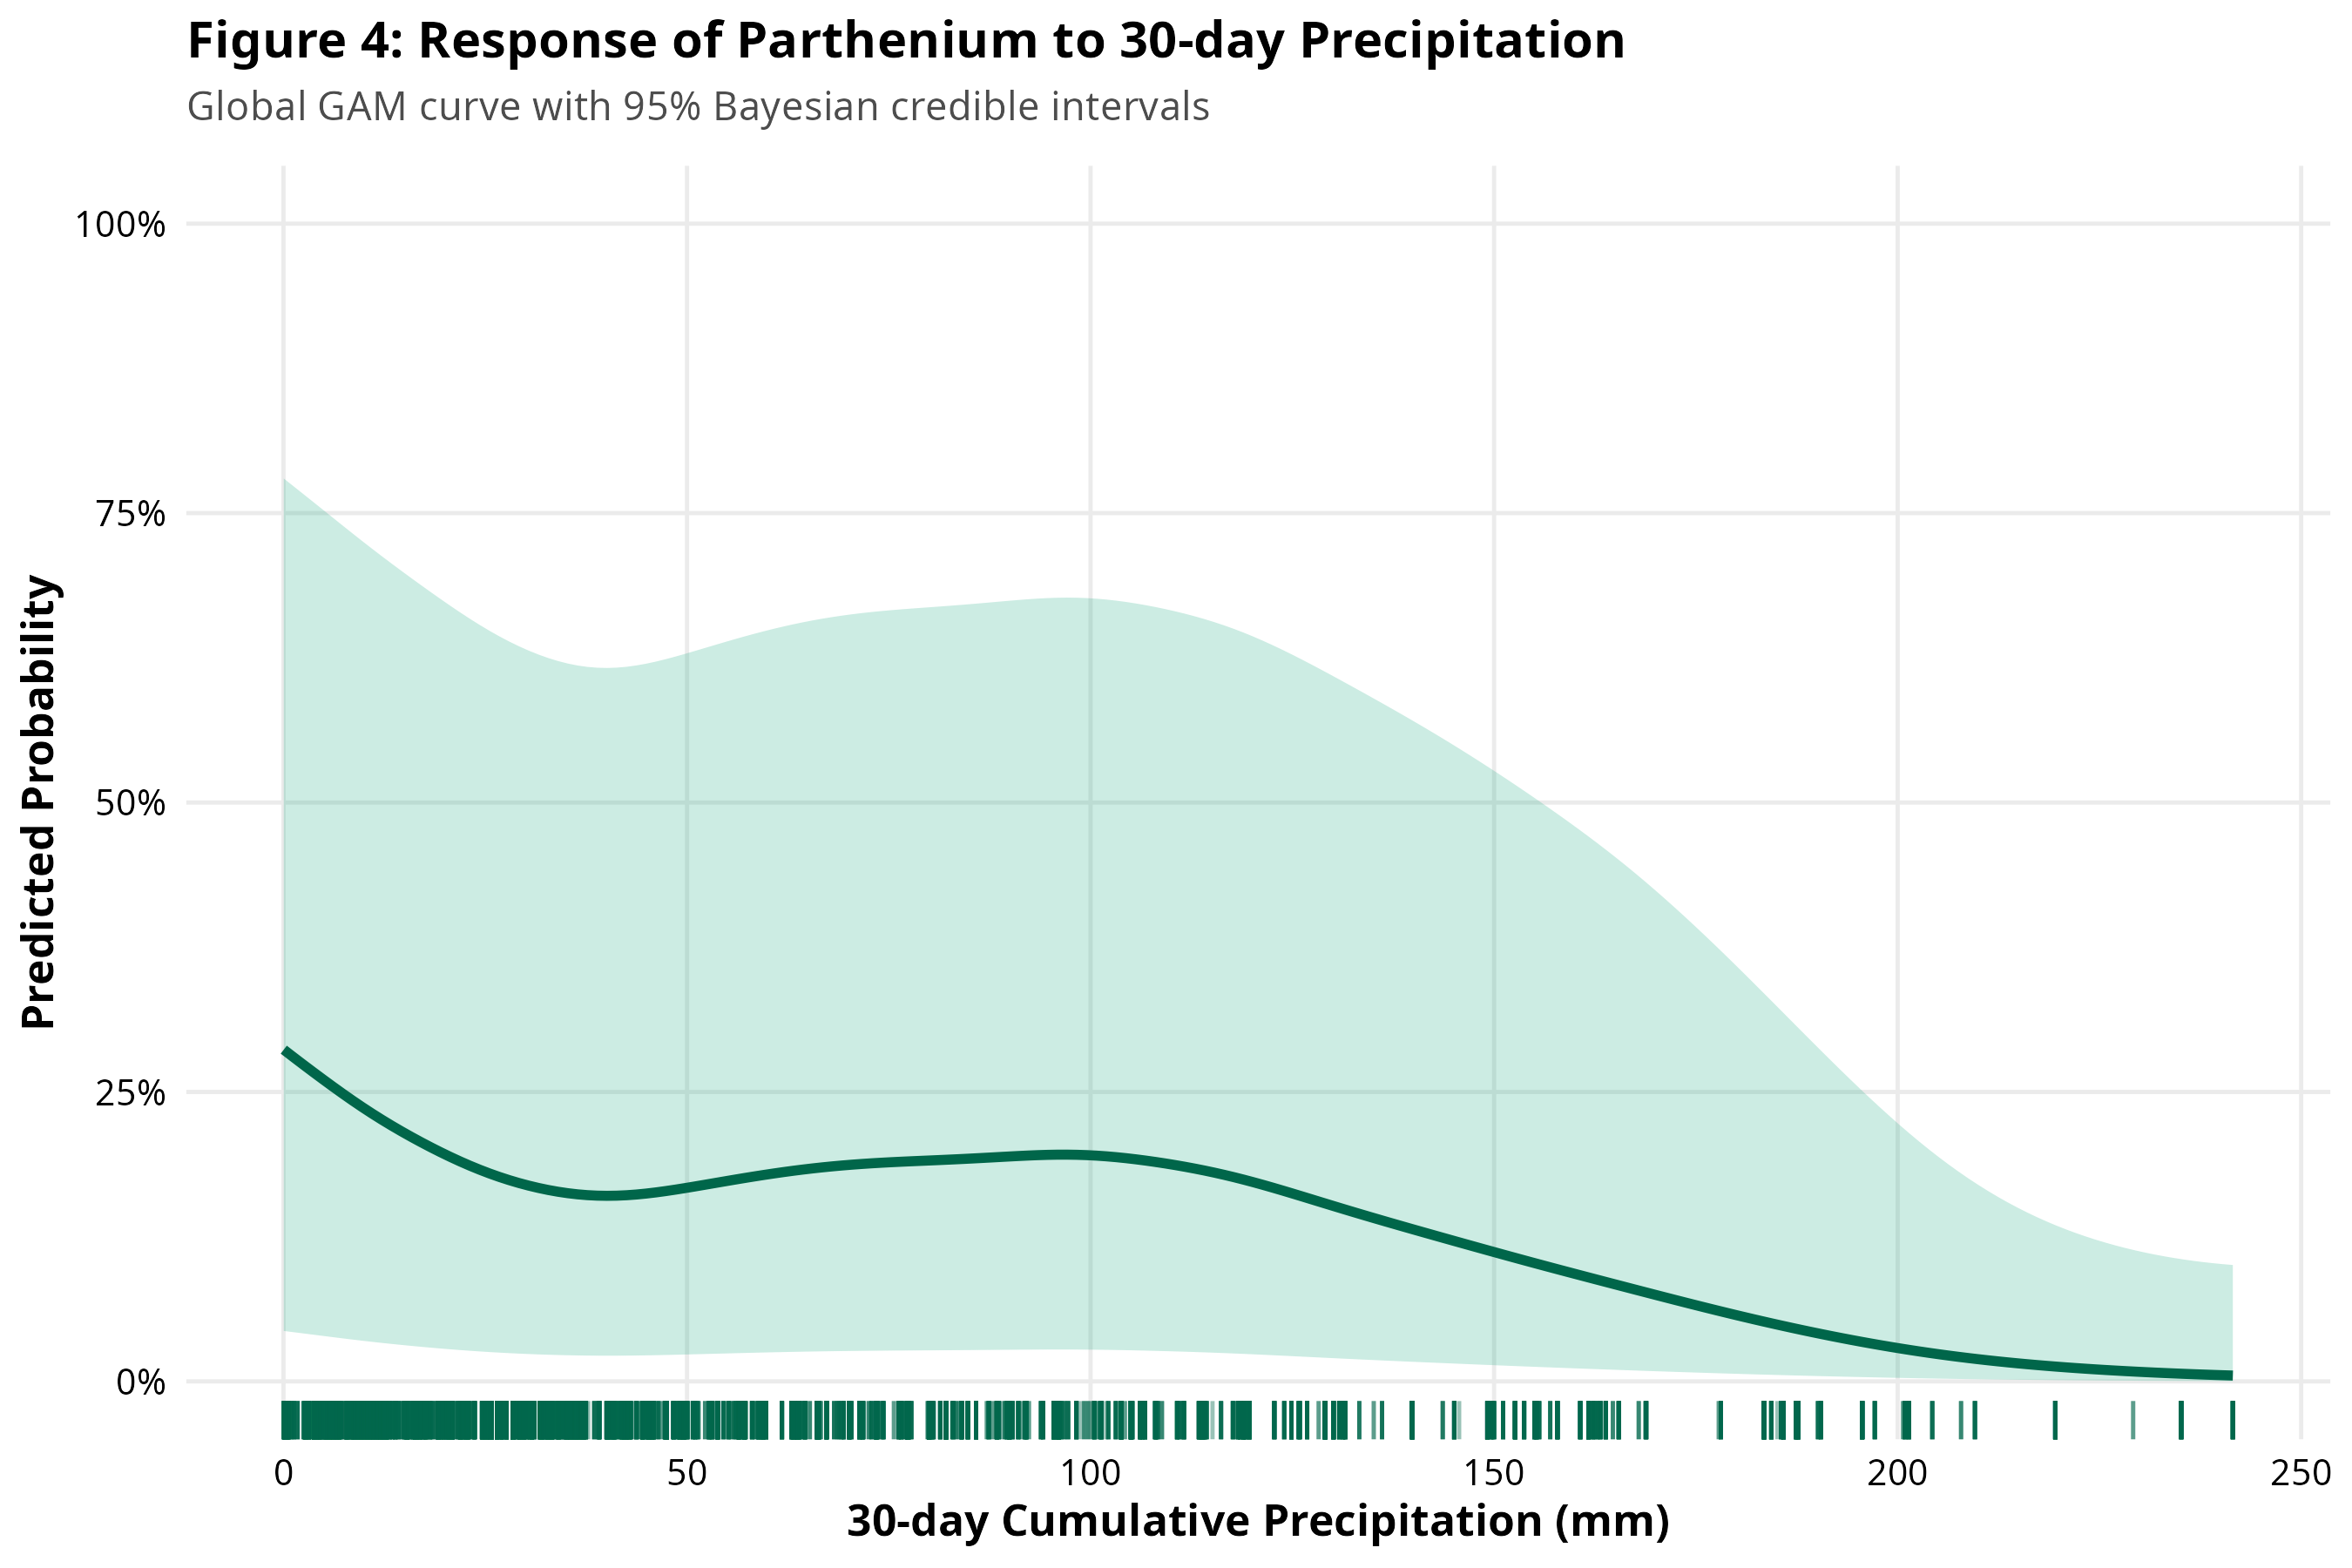
\includegraphics[width=\textwidth]{figures/fig4_precipitation_smooth.png}
    \caption{Partial response curve of \textit{Parthenium hysterophorus} occurrence probability to 30-day cumulative precipitation (mm). The solid line represents the expected partial smooth effect from model \texttt{M5\_k200} with secondary covariates held constant; the shaded ribbon depicts 95\% confidence intervals. Widened confidence bands at low precipitation thresholds ($< 25$ mm) reflect domain edge uncertainty and sparse observation density.}
    \label{fig:precip-response}
\end{figure}

\section{Forecasting and biocontrol thermal suitability (India, 2030/2050)}

Figure~\ref{fig:india-projections} presents projected climatic suitability for \textit{Parthenium hysterophorus}, the thermal suitability proxy for \textit{Zygogramma bicolorata}, and their spatial overlap across India under present, 2030, and 2050 climate scenarios. A lower \textit{Parthenium} threshold was used to capture marginally suitable areas that may represent early-warning invasion pathways. The \textit{Zygogramma} layer represents broad thermal-climatic permissiveness rather than direct predictions of beetle establishment or biocontrol efficacy.

MaxEnt projections indicated that \textit{Parthenium} suitability is extensive under current conditions but becomes increasingly restricted and fragmented under future scenarios. In contrast, the annual temperature-based \textit{Zygogramma} proxy remained high across most of India, indicating persistent annual thermal permissiveness despite warming. Using thresholds of 0.4952 for \textit{Parthenium} and 0.75 for \textit{Zygogramma}, jointly suitable cells declined from 66.0\% under current conditions to 42.0\% in 2030 and 20.6\% in 2050. Beetle-only cells increased from 30.4\% to 55.8\% and 77.5\%, respectively, while \textit{Parthenium}-only cells remained negligible. Thus, declining overlap was primarily driven by contraction of \textit{Parthenium} suitability rather than loss of annual beetle thermal suitability.

Despite the permissive \textit{Parthenium} threshold, future climate projections did not produce a broad national-scale area where \textit{Parthenium} suitability exceeded the beetle proxy. However, the 2050 summer heat-stress panel provides an important seasonal contrast: although annual conditions remain broadly permissive for \textit{Zygogramma}, large areas may experience temperatures approaching or exceeding its upper thermal limits. This indicates that seasonal heat stress may impose constraints not captured by the annual thermal proxy.

\begin{figure}[H]
    \centering
    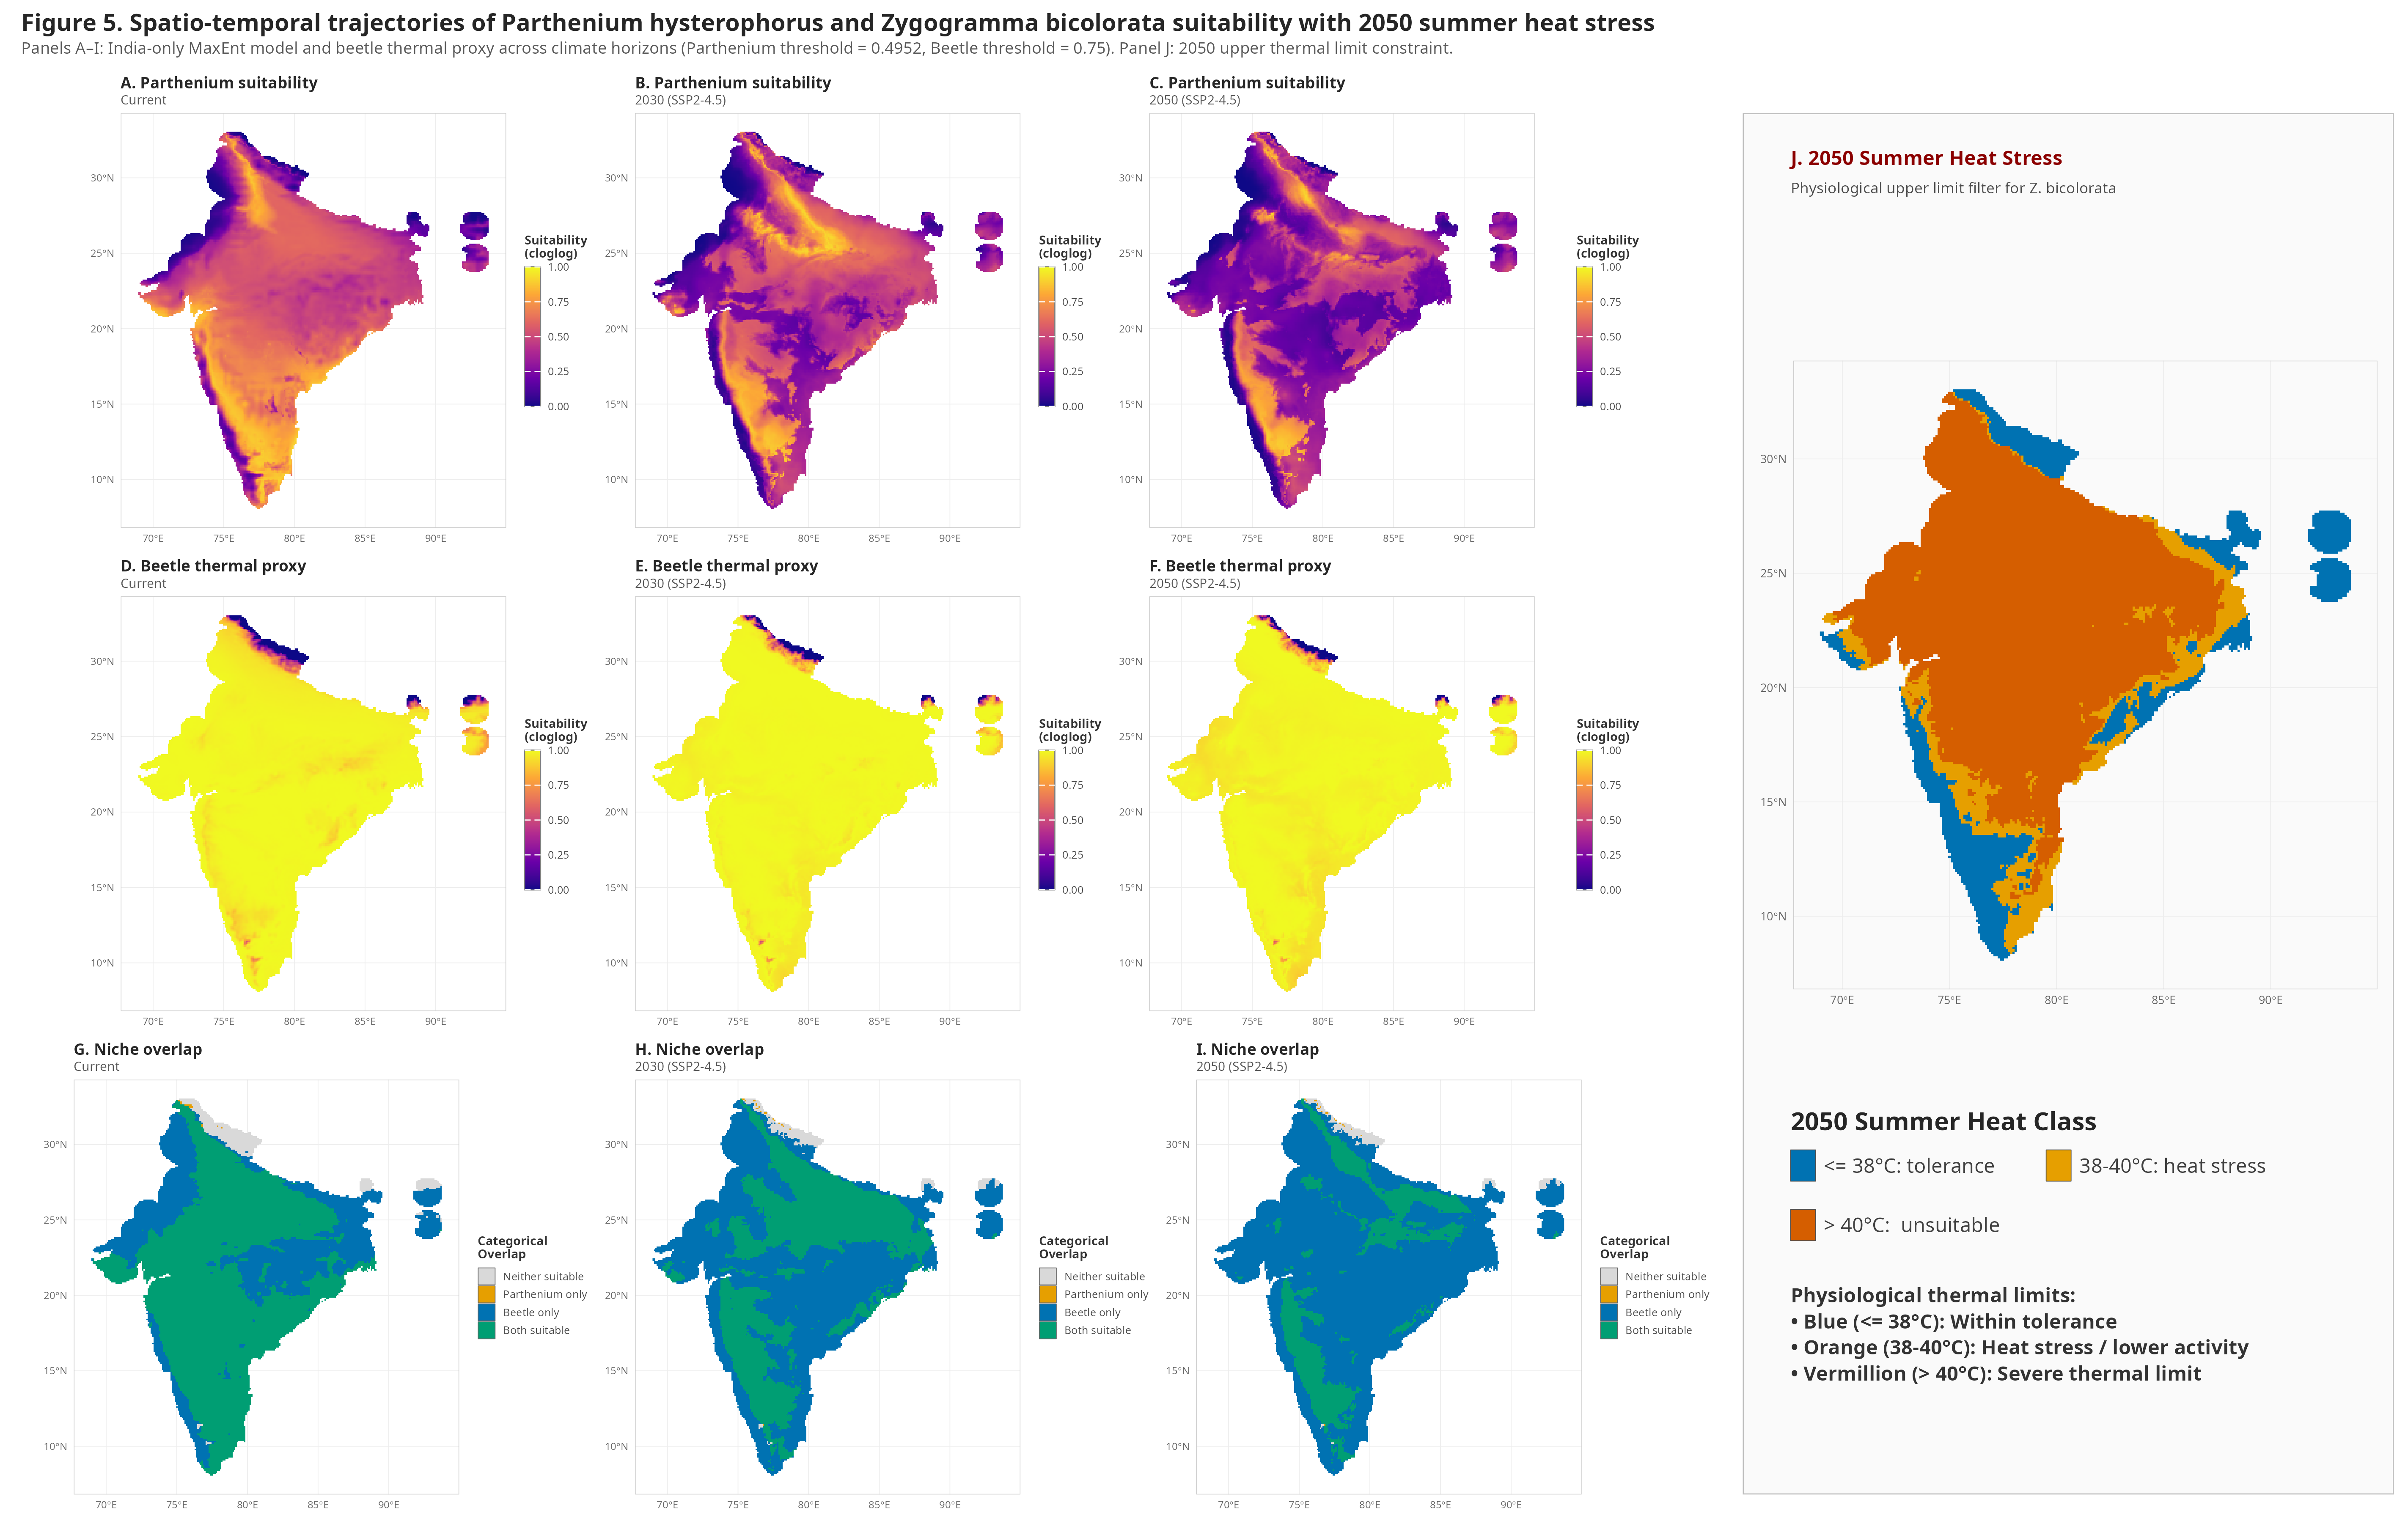
\includegraphics[width=\textwidth]{figures/fig5_india_projections.png}
    \caption{India-only projections of \textit{Parthenium} suitability, beetle thermal suitability, overlap, and supporting 2050 summer heat stress. Panels A--C show climatic suitability for \textit{Parthenium hysterophorus} predicted from the India-only MaxEnt/maxnet model for the current period, 2030, and 2050. Panels D--F show a thermal suitability proxy for the beetle based on annual mean temperature using a temperature-response function with Tmin = 10$^{\circ}$C, Topt = 27$^{\circ}$C, and Tmax = 38$^{\circ}$C. Panels G--I show categorical overlap between \textit{Parthenium} suitability and beetle thermal suitability, classified using thresholds of 0.4952 for \textit{Parthenium} and 0.75 for the beetle proxy. Overlap classes indicate areas suitable for neither, \textit{Parthenium} only, beetle only, or both. The supporting panel (J) shows 2050 maximum summer temperature classified according to beetle upper thermal limits: $\leq 38^{\circ}$C = within broad tolerance, 38--40$^{\circ}$C = heat stress, and $> 40^{\circ}$C = likely unsuitable for sustained summer survival. The beetle layer should be interpreted as a broad climatic thermal proxy rather than a separate occurrence-based species distribution model.}
    \label{fig:india-projections}
\end{figure}

\section{Spatial model comparison}

A comparison of spatial projections from the Pakistan-calibrated GAM and the India-calibrated MaxEnt models revealed only partial concordance across Pakistan (Figure~\ref{fig:pakistan-concordance}). Analysis of 7{,}246 overlapping grid cells revealed a weak association (Spearman's $\rho = 0.295$; Pearson's $r = 0.143$). Both models captured broad spatial trends but differed substantially in location-specific suitability.

The two continuous suitability surfaces showed broadly different spatial structures (Figure~\ref{fig:pakistan-concordance}A--B). The GAM identified southern and south-eastern Pakistan as most suitable, with suitability declining northward. MaxEnt also favoured southern Pakistan but showed greater heterogeneity, with high suitability extending into western and central areas. Both models showed a south-to-north decline, but MaxEnt emphasised more internal spatial variation.

Model agreement on the hotspot areas of predicted suitability was modest, suggesting only a quarter of top-suitability cells overlapped (Jaccard index = 0.251; Figure~\ref{fig:pakistan-concordance}C). Shared high-suitability zones clustered in southern Pakistan (notably the lower Indus), while the GAM highlighted the southern and south-eastern lowlands and MaxEnt emphasised the west and south-west.

The continuous rank-difference surface (Figure~\ref{fig:pakistan-concordance}D) confirmed spatially structured disagreement. Cells ranked higher by the GAM clustered in the south and east, while those favoured by MaxEnt were in the west and central Pakistan. These patterns indicate that the models were not simply differing in prediction intensity, but were prioritising different regions of environmental space when projected across Pakistan.

In summary, the MaxEnt and GAM models captured some broad-scale suitability patterns but showed limited agreement on high-suitability areas. Model choice and calibration geography strongly influence projected suitability, affecting transferability and spatial prioritisation.

\begin{figure}[H]
    \centering
    \includegraphics[width=\textwidth]{figures/fig6_pakistan_concordance.png}
    \caption{Spatial concordance between the Pakistan-calibrated GAM and the India-calibrated MaxEnt projection across Pakistan. (A) Relative suitability predicted by the Pakistan-calibrated GAM. (B) Relative suitability predicted by the India-calibrated MaxEnt model projected onto Pakistan. (C) Categorical spatial concordance based on the upper quartile of predictions from each model, showing cells classified as both low, GAM-only high, MaxEnt-only high, or both high. Relative suitability in panels A and B is shown as within-model percentile rank to allow comparison of spatial pattern rather than absolute prediction magnitude. Concordance was calculated from 7{,}246 overlapping cells. (D) Model divergence map highlighting where models disagree most.}
    \label{fig:pakistan-concordance}
\end{figure}
\chapter{Discussion}

The model selection results highlight the pivotal influence of spatial structure and environmental variables on \textit{Parthenium hysterophorus} distribution in Pakistan. Adding spatial smooth terms greatly improved model fit, evidenced by higher deviance explained and lower AIC, demonstrating that accounting for spatial autocorrelation is critical, as non-spatial models performed poorly by comparison.

While environmental predictors are important, they do not fully explain distribution patterns. Notably, increasing the spatial smooth basis from $k = 100$ to $k = 200$ substantially enhanced the model's ability to capture fine-scale spatial variation, suggesting that \textit{Parthenium}'s distribution is shaped by complex, geographically structured factors beyond those measured. Even after including key variables, altitude, climate, habitat, and road type, a significant residual spatial component persisted, as shown by the strong Gaussian process smooth. This suggests unmeasured or spatially structured drivers, such as local land use, dispersal dynamics, or microclimate, also play important roles and merit further study [X].

Altitude and road type were especially influential predictors, with model performance declining notably when either was excluded. The importance of road type is consistent with literature showing that transportation networks promote invasive species spread by offering dispersal corridors and disturbance regimes [X]. These insights underscore the need for targeted management along roadways and in vulnerable habitats [X].

The final REML-fitted GAM explained over 60\% of the deviance, confirming strong explanatory power. Yet, substantial residual spatial structure remains even after accounting for environmental and anthropogenic variables, indicating that other, finer-scale factors may influence distribution. Future research should incorporate higher-resolution spatial data, additional ecological covariates, and biotic interactions to clarify these drivers. Exploring \textit{Parthenium}'s use of allelochemicals to gain pollinator preference and enhance spread may also reveal important survival mechanisms [X].

The GAM results reveal that \textit{Parthenium hysterophorus} occurrence is primarily determined by the interplay of habitat disturbance, transport infrastructure, and climatic conditions [X]. The species is most likely to occur in open, disturbed habitats and along major road corridors, highlighting the strong association between invasion risk, land-use intensity, and human-mediated dispersal. Additionally, the notable nonlinear effects of climatic variables indicate that invasion is governed not just by disturbance, but by how these opportunities intersect with environmental suitability.

Habitat type is a major driver of invasion risk for \textit{P. hysterophorus}. Disturbed and unmanaged open habitats have the highest baseline occurrence, supporting the view of \textit{P. hysterophorus} as a classic disturbance-adapted pioneer species [X]. These plants quickly colonise areas where vegetation is disrupted, competition is low, and direct soil contact is possible. Following Grime's ecological framework, \textit{Parthenium} exhibits pioneer traits by prioritising rapid growth, flowering, and prolific seed production over long-term competition [X]. Agricultural Disturbed and Semi-natural Open habitats create especially favourable conditions with frequent disturbances, exposed soil, and resource pulses [X]. Such settings may also allow contaminants to affect soil composition and fertility, especially without biological fertilisers or other management interventions [X]. By contrast, habitats with active management or stronger natural resistance, such as Agricultural Managed land, Woody Vegetation, and Wet Habitats, exhibit much lower occurrence, indicating that both human control and biophysical barriers can suppress \textit{Parthenium} establishment.

Lower occurrence in managed and structurally complex habitats provides further ecological insight. In actively managed agricultural systems, repeated interventions, such as weed control, crop rotation, and maintaining managed ground, reduce establishment opportunities for \textit{Parthenium}. In woody vegetation, closed canopies limit light and established perennial species increase competition, collectively suppressing \textit{Parthenium} growth [X]. In wet habitats, excess moisture or related ecological factors may constrain invasion, either by directly causing physiological stress to \textit{Parthenium} or by enhancing competition from moisture-adapted plant communities [X]. These patterns illustrate how both management practices and natural habitat complexity serve as effective barriers to invasion.

Recent thermal accumulation, measured as 30-day growing degree days (GDD), was a strong but nonlinear predictor of \textit{Parthenium hysterophorus} occurrence. Rather than increasing steadily with temperature, occurrence peaked at intermediate to upper-intermediate GDD levels, particularly in less-managed habitats. This likely reflects the temperature dependence of multiple life stages, including germination, growth, flowering, and seed production, each with different optimal conditions [X]. Temperature therefore influences seasonal opportunities for establishment and spread, while excessive heat may cause sun bleaching, reducing photosynthesis and limiting growth and reproduction [X].

The bimodal or trimodal GDD pattern likely reflects seasonal rather than multiple discrete physiological optima. Occurrence peaked in August, with a secondary increase in November, while cooler months showed lower occurrence. These peaks may represent periods favourable for establishment and reproduction, with August corresponding to the main growth phase and November potentially reflecting secondary recruitment or post-monsoon persistence [X]. However, the apparent peaks should not be interpreted as sharp biological thresholds. Sparse observations and wide confidence intervals at thermal extremes increase uncertainty, and GAMs can produce exaggerated curvature where data are limited [X]. Interpretation should therefore focus on the better-sampled central portion of the gradient.

More broadly, GDD represents only one component of the \textit{P. hysterophorus} invasion niche. Moisture, disturbance, irrigation, hydrology, vegetation, and land management also influence occurrence and may covary with temperature [X]. Precipitation showed a nonlinear association, with occurrence highest under low-to-moderate rainfall and declining under wetter conditions. Thus, \textit{P. hysterophorus} appears most favoured where warmth coincides with intermediate moisture, particularly in open, disturbed habitats [X].

This distinction is also important for future projections. Under the current temperature-based model, \textit{Zygogramma bicolorata} remains broadly within climatic tolerance across India, while \textit{Parthenium} suitability contracts by 2050. However, the model excludes hydrological buffering. Irrigation studies in Pakistan show that incorporating water availability can substantially increase predicted \textit{Parthenium} suitability, particularly in marginal areas [X]. Temperature-only projections may therefore overestimate future declines where moisture offsets thermal stress [X].

Model forecasts indicate that, under the current assumptions, the beetle largely remains within climatic tolerance across India, while suitable climate for \textit{Parthenium hysterophorus} contracts over time. This apparent beetle resilience reflects the permissive annual thermal proxy used. By 2050, reduced overlap is primarily driven by declining \textit{Parthenium} suitability as temperatures exceed physiological thresholds that may impair metabolic processes and persistence [X]. These projections should therefore be interpreted as baseline thermal risk assessments rather than comprehensive ecological forecasts.

However, the temperature-only model omits key environmental drivers, particularly precipitation and moisture, which can buffer heat stress and support persistence under otherwise unsuitable temperatures. Irrigation studies in Pakistan show that incorporating water availability can substantially increase predicted \textit{Parthenium} suitability, particularly in marginal areas [X]. Temperature-only projections may therefore overestimate future declines where hydrological buffering occurs [X].

The 2050 heat-stress panel provides an important seasonal perspective, revealing thermal bottlenecks obscured by annual averages. Although annual conditions remain broadly permissive for \textit{Zygogramma bicolorata}, large areas of central and southern India may experience summer temperatures associated with heat stress or thermal unsuitability, potentially limiting beetle persistence before the monsoon [X]. Cooler regions, particularly the northeast and areas below 38$^{\circ}$C, may provide thermal refugia. However, these projections use coarse macroclimatic data and do not capture cooler microclimates provided by shaded foliage or moist soils [X].

The heat-stress assessment also excludes monsoon timing, soil moisture, diapause, and seasonal emergence dynamics, all of which influence \textit{Z. bicolorata} persistence. In addition, real-world biocontrol involves dynamic ecological feedbacks: beetle populations may increase following \textit{Parthenium} expansion but subsequently decline as food resources are depleted, while predators, parasitoids, and phenological mismatches may further constrain control [X] [X]. Accordingly, the figure provides a broad macroclimatic assessment rather than a process-based biocontrol forecast. Its main contribution is to identify temperature as an important constraint, highlight potential future narrowing of weed--beetle overlap, and demonstrate that summer heat extremes may create bottlenecks that annual climate averages overlook [X].

Comparison of the Pakistan-calibrated GAM and India-calibrated MaxEnt models revealed only partial spatial agreement across Pakistan. Weak positive correlations (Spearman's $\rho$; Pearson's $r$) indicate that the models differ in both rank ordering and predicted suitability, despite being compared across the same spatial support.

This divergence likely reflects differences in calibration domain, predictors, model framework, and data. The GAM was calibrated using Pakistani data, whereas MaxEnt was trained on Indian data and transferred to Pakistan, meaning the models represent different environmental and realised-niche relationships. MaxEnt uses broad climatic predictors, while the GAM incorporates growing degree days, precipitation, altitude, and habitat cover. The GAM also restricted projections to its training environmental envelope and excluded spatial smoothing to minimise unsupported extrapolation. Differences between controlled presence--absence data for Pakistan and presence-only data with varying sampling bias for India may further contribute to the contrasting suitability surfaces.

Despite weak overall concordance, both models identified a shared southern hotspot. Areas classified as ``both high'' therefore provide more robust candidate regions because they are supported across two independent calibration contexts. In contrast, ``GAM only high'' and ``MaxEnt only high'' areas represent model uncertainty and may reflect differences in predictor sensitivity, local environmental structure, or extrapolation [X].

The low Jaccard overlap among the top 25\% of suitability cells reinforces that hotspot identification is model-dependent. However, comparison on an identical aligned valid-cell set and use of relative suitability ranks improve comparability between models. The rank-difference surface further identifies where each model assigns greater suitability [X].

Overall, Figure~\ref{fig:pakistan-concordance} demonstrates that transferred MaxEnt predictions capture some, but not all, of the spatial pattern identified by the Pakistan-calibrated GAM. Areas of agreement provide useful targets for future validation, while divergent regions highlight uncertainty and the limitations of transferring models across calibration geographies [X].

\section{Conclusion}

Overall, the GAM captured fine-scale, season- and habitat-linked occurrence risk, while MaxEnt identified broader climatic gradients. Both models highlighted disturbed, warmer, invasion-prone areas, but differed in hotspot locations and extent, underscoring that \textit{Parthenium} favours specific environments requiring further investigation. For management, derelict lands, semi-natural open habitats, and disturbed agricultural areas should be prioritised for surveillance and control, with interventions timed to peak seasonal windows and guided by real-time climate data [X]. Public awareness remains limited: hand-pulling is common in small fields, but knowledge of biocontrol is low [X]. Broader dissemination of biocontrol information and stronger prevention policies, such as stricter border and transport surveillance, are needed [X]. Given that conflict and increased transport may accelerate seed dispersal across South Asia, management must address both anthropogenic pathways and climatic suitability. Species distribution models remain scenario-based approximations, limited by predictor choice and unable to fully resolve dispersal, biotic interactions, microclimate, or feedback [X]. Nevertheless, this study provides a crucial spatial baseline for assessing climatic risk, identifying management priorities, and guiding research on how warming may affect \textit{Parthenium} and its biocontrol agent in Pakistan [X].

% Data and code statement before bibliography, per guidance
\cleardoublepage
\chapter*{Data and Code Availability}
\addcontentsline{toc}{chapter}{Data and Code Availability}

The data and code supporting this dissertation will be archived in a public or supervised-access repository before final submission, subject to any permissions, confidentiality constraints, and collaborator agreements applying to survey or derived spatial datasets.

Pakistan roadside survey data, derived environmental layers, modelling scripts, and figure-generation workflows will be made available in a form sufficient to support replication of the principal analyses where permitted. India occurrence records were compiled from public biodiversity databases and processed for modelling as described in the Methods chapter. Climate layers were derived from ERA5-Land and associated processed raster workflows.

Where full public release is not possible, this will be clearly stated in the final submitted version together with the reason for restriction and, where appropriate, a route by which eligible researchers may request access.

% Supplementary material / appendices
\appendix
\chapter{Supplementary Material}

This appendix contains supplementary material supporting the main dissertation. It may include:
  
  \begin{itemize}
\item additional model-selection tables and diagnostics;
\item software versions and package details;
\item sensitivity analyses;
\item supplementary figures and extended methods;
\item additional notes on preprocessing and projection workflows.
\end{itemize}

Add supplementary tables, figures, or extended methods below as needed.

\cleardoublepage
\RemoveLabels
\thesisspacing
\printbibliography[title={Bibliography},heading=bibintoc]

\end{document}
